\subsection{Red Laboratorios DC}

Para el último experimento, capturamos los paquetes de la LAN Wi-Fi Laboratorios-DC del Departamento de Computació de la FCEyN de la UBA. La medición fue realizada un día Lunes desde las 15hs y durante 15 minutos. La cantidad de paquetes capturados es de 19.000. De todos estos, sólo 974 corresponden al protocolo ARP.

\subsubsection{Descripción}

El siguiente experimento consistió en medir la LAN Wi-Fi pública del shopping Alto Palermo. Esta medición se llevó a cabo un día Sábado a las 21hs, con un tiempo de medición fue de aproximádamente 40 minutos y se capturaron 1569 paquetes ARP, de los cuales 687 eran de tipo \emph{who-has}.

A continuación mostramos un grafo que muestra los nodos de la red con su dirección IP y la cantidad de mensajes de tipo \emph{who-has}.

%\begin{figure}[H]
% \begin{center}
%  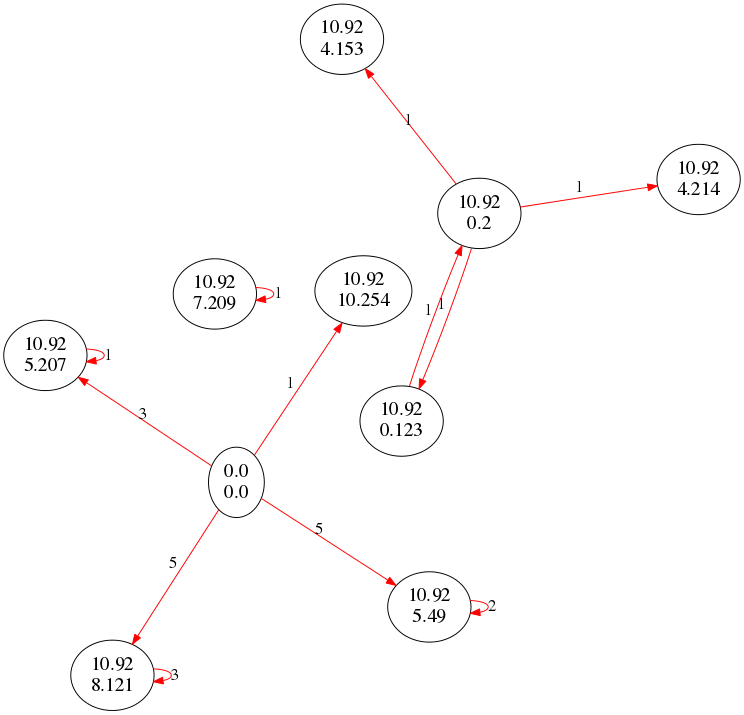
\includegraphics[width=0.9\linewidth]{/home/pato/workspace/TP1-Redes/informe/imgs/red_dc/network.png}
%  \caption{Grafo Medición DC}
% \end{center}
%\end{figure}

Como podemos ver en el grafo, la red tiene dos nodos que se destacan. Uno de estos nodos, el cual tiene la dirección IP \emph{117.17.12.1}, recibe muchos paquetes de la mayoría de los otros nodos de la red, pero no envía ninguno. Y el otro, con dirección IP \emph{117.17.12.2} recibe varios paquetes y también envía varios.

También podemos observar que hay un nodo con dirección \emph{0.0.0.0}, el cual envía varios mensajes. %TODO explicar qué es el 0.0.0.0

\subsubsection{Fuente: Destino}


\subsubsection{Fuente: Origen}



\subsubsection{Discusión}
